\documentclass{beamer}
\usepackage[utf8]{inputenc}

\usetheme{Madrid}
\usecolortheme{default}
\usepackage{amsmath,amssymb,amsfonts,amsthm}
\usepackage{txfonts}
\usepackage{tkz-euclide}
\usepackage{listings}
\usepackage{adjustbox}
\usepackage{array}
\usepackage{tabularx}
\usepackage{gvv}
\usepackage{lmodern}
\usepackage{circuitikz}
\usepackage{tikz}
\usepackage{graphicx}

\setbeamertemplate{page number in head/foot}[totalframumber]

\usepackage{tcolorbox}
\tcbuselibrary{minted,breakable,xparse,skins}



\definecolor{bg}{gray}{0.95}
\DeclareTCBListing{mintedbox}{O{}m!O{}}{%
  breakable=true,
  listing engine=minted,
  listing only,
  minted language=#2,
  minted style=default,
  minted options={%
    linenos,
    gobble=0,
    breaklines=true,
    breakafter=,,
    fontsize=\small,
    numbersep=8pt,
    #1},
  boxsep=0pt,
  left skip=0pt,
  right skip=0pt,
  left=25pt,
  right=0pt,
  top=3pt,
  bottom=3pt,
  arc=5pt,
  leftrule=0pt,
  rightrule=0pt,
  bottomrule=2pt,
  toprule=2pt,
  colback=bg,
  colframe=orange!70,
  enhanced,
  overlay={%
    \begin{tcbclipinterior}
    \fill[orange!20!white] (frame.south west) rectangle ([xshift=20pt]frame.north west);
    \end{tcbclipinterior}},
  #3,
}
\lstset{
    language=C,
    basicstyle=\ttfamily\small,
    keywordstyle=\color{blue},
    stringstyle=\color{orange},
    commentstyle=\color{green!60!black},
    numbers=left,
    numberstyle=\tiny\color{gray},
    breaklines=true,
    showstringspaces=false,
}
%------------------------------------------------------------
%This block of code defines the information to appear in the
%Title page
\title %optional
{4.2.5}
\date{October 6,2025}
%\subtitle{A short story}

\author % (optional)
{EE25BTECH11002 - Achat Parth Kalpesh}



\begin{document}

\frame{\titlepage}

\begin{frame}{Question}
Find the direction and normal vector for the line;
\begin{align}
    2x=-5y
    \label{eq:ref}
\end{align}
\end{frame}

\begin{frame}{Theoretical Solution}
Let $\vec{n}$ and $\vec{m}$ are the Normal and Direction vectors of the 
line
\begin{align}
    \vec{n_1}^\top\vec{x}=c
\end{align}
where ,
\begin{align}
    \vec{n_1} &= \myvec{2 \\ 5}\\
    c &= 0
\end{align}

\end{frame}

\begin{frame}{Theoretical Solution}
The $\vec{n}$ can be represented as,
\begin{align}
    \vec{n} = \myvec{-m \\ 1}
\end{align}
Where $m$ is the slope of the line,
\begin{align}
    m &= \frac{-2}{5}\\
    \vec{n} &= \myvec{\frac{2}{5} \\ 1}
\end{align}

\end{frame}

\begin{frame}{Theoretical Solution}
\eqref{eq:ref} can be represented as,
\begin{align}
    \implies \myvec{x \\ y} &= \myvec{x \\ \frac{-2}{5}x} =\myvec{0 \\ 0} + x\myvec{1 \\ \frac{-2}{5}}\\
    \implies \myvec{x \\ y} &=\myvec{0 \\ 0} + x\myvec{1 \\ \frac{-2}{5}}
\end{align}
Comparing it with ,
\begin{align}
\label{eq:geo-param}
	\vec{x} = \vec{h} + \kappa \vec{m}
\end{align}
We get,
\begin{align}
			\label{eq:line-school-dir}
\vec{m} = \myvec{1 \\ \frac{-2}{5}}
\end{align}
\end{frame}

\begin{frame}[fragile]
    \frametitle{C code}
    \begin{lstlisting}
#include <stdio.h>
void formula(double *a,double *b)
{
   double x, y;
   a[0] = a[0]/a[1];
   a[1] = 1;
   b[0] = 1;
   b[1] = -a[0]; 
}
    \end{lstlisting}
\end{frame}

\begin{frame}[fragile]
    \frametitle{Python Code}
    \begin{lstlisting}[language=Python]
import numpy as np
import matplotlib.pyplot as plt
import ctypes
lib_path = ctypes.CDLL('./formula.so')
lib_path.formula.argtypes = [
    ctypes.POINTER(ctypes.c_float)
]
lib_path.formula.restype = ctypes.c_float
# The equation of the line is 2x = -5y, which can be rewritten as 2x + 5y = 0.

# --- 1. Define the Normal and Direction Vectors ---
# For a line Ax + By + C = 0, the normal vector is (A, B).
normal_vector = np.array([2, 5])

# The direction vector is perpendicular to the normal vector.
# If n = (A, B), the direction vector d can be (-B, A).
direction_vector = np.array([-5, 2])
    \end{lstlisting}
\end{frame}

\begin{frame}[fragile]
    \frametitle{Python Code}
    \begin{lstlisting}[language=Python]
# --- 2. Generate points to plot the line ---
# From the equation 2x + 5y = 0, we can express y as y = (-2/5)x.
# We will generate a set of x-values to find the corresponding y-values.
x_vals = np.linspace(-10, 10, 100)
y_vals = (-2/5) * x_vals

# --- 3. Create the plot ---
plt.figure(figsize=(9, 9))
ax = plt.gca()

# Plot the line itself
plt.plot(x_vals, y_vals, label='Line: 2x + 5y = 0', color='blue', zorder=1)

# Plot the normal and direction vectors starting from the origin (0,0)
# We use plt.quiver to draw arrows.
    \end{lstlisting}
\end{frame}

\begin{frame}[fragile]
    \frametitle{Python Code: Plotting}
    \begin{lstlisting}[language=Python]
origin = [0], [0]
plt.quiver(*origin, normal_vector[0], normal_vector[1], 
           angles='xy', scale_units='xy', scale=1, 
           color='red', label=f'Normal Vector: [0.4 , 1]')
plt.quiver(*origin, direction_vector[0], direction_vector[1], 
           angles='xy', scale_units='xy', scale=1, 
           color='green', label=f'Direction Vector: [1 , -0.4]')


# --- 4. Format the plot for clarity ---
# Set the limits for the x and y axes
plt.xlim(-10, 10)
plt.ylim(-10, 10)

# Ensure the aspect ratio is equal, so perpendicular lines look correct
plt.axis('equal')
    \end{lstlisting}
\end{frame}

\begin{frame}[fragile]
    \frametitle{Python Code: Finalizing Plot}
    \begin{lstlisting}[language=Python]
# Move the x and y axes to the center to mimic a Cartesian plane
ax.spines['left'].set_position('zero')
ax.spines['bottom'].set_position('zero')
ax.spines['right'].set_color('none')
ax.spines['top'].set_color('none')

# Add labels, a title, a legend, and a grid
plt.xlabel('x-axis', fontsize=12)
plt.ylabel('y-axis', fontsize=12, rotation=0)
ax.xaxis.set_label_coords(1.05, 0.51)
ax.yaxis.set_label_coords(0.51, -0.05)
plt.title('Direction and Normal Vector for the Line 2x = -5y', fontsize=14)
plt.legend(loc='best')
plt.grid(True)
plt.savefig('./fig.jpg')
# Display the plot
plt.show()
    \end{lstlisting}
\end{frame}

\begin{frame}{Plot}
    \begin{figure}
        \centering
        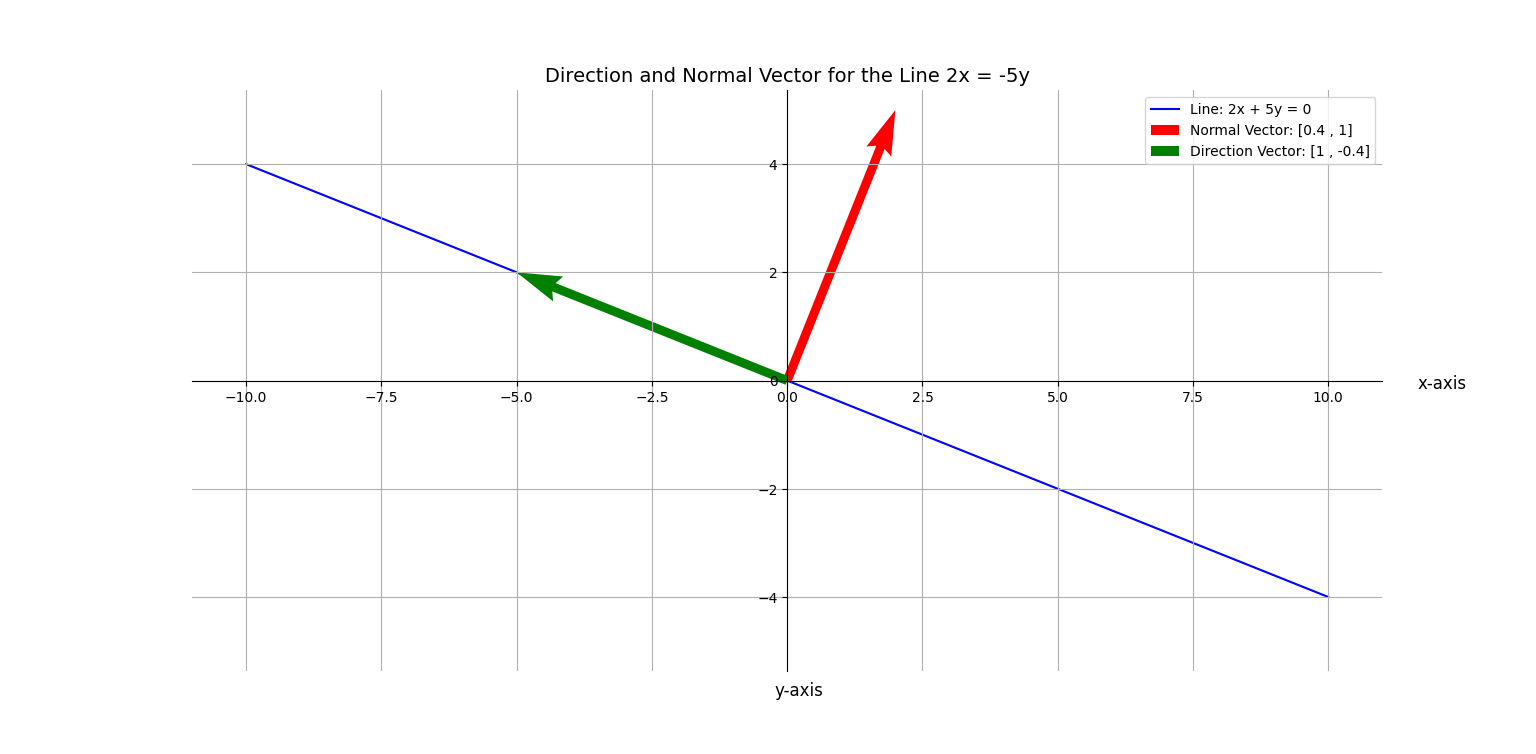
\includegraphics[width=\columnwidth]{../figs/figure_py.png}
        \caption{Direction and Normal Vector for the Line 2x = -5y}
        \label{fig:final_plot}
    \end{figure}
\end{frame}

\end{document}
